\documentclass[12pt,twoside]{article}
\usepackage{amsmath, amssymb}
\usepackage[active]{srcltx}
\usepackage{amssymb}
\usepackage{amscd}
\usepackage{makeidx}
\usepackage{amsthm}
\usepackage{algorithm}
\usepackage{algpseudocode}
\usepackage{wrapfig,lipsum}

\usepackage{fancyhdr}
\usepackage{graphics}
%----------------------------------------------------------------------------------------------
\usepackage{amsmath, amssymb}
\usepackage{amsmath}
\usepackage[active]{srcltx}
\usepackage{amssymb}
\usepackage{amscd}
\usepackage{makeidx}
\usepackage[dvips]{graphicx}
\usepackage{latexsym}

\renewcommand{\baselinestretch}{1}
\setcounter{page}{1}
\setlength{\textheight}{21.6cm}
\setlength{\textwidth}{14cm}
\setlength{\oddsidemargin}{1cm}
\setlength{\evensidemargin}{1cm}
\pagestyle{myheadings}
\thispagestyle{empty}
\markboth{\small{Pr\'actica 2. Anthony Steiner.}}{\small{.}}
\date{}
\begin{document}

\begin{figure}[h]
\vspace{-3cm} \hspace{-2cm} \setlength{\unitlength}{1mm}
\begin{picture}(15,25)(-10,0)

\includegraphics[width=16cm,height=3cm]{titulo.jpg}
\end{picture}
\end{figure}

\vspace{0cm}

\centerline{\bf An\'alisis de Algoritmos, Sem: 2022-2, 3CV11, Pr\'actica 2, 14/03/2022}

\centerline{}

%\centerline{}

\begin{center}
\Large{\textsc{Pr\'actica 2: Complejidades temporales polinomiales y no polinomiales.}}
\end{center}
\centerline{}
\centerline{\bf {Steiner V\'azquez Anthony Francis}}
\centerline{}
\centerline{$asteinerv1700@alumno.ipn.mx$}


\newtheorem{Theorem}{\quad Theorem}[section]

\newtheorem{Definition}[Theorem]{\quad Definition}

\newtheorem{Corollary}[Theorem]{\quad Corollary}

\newtheorem{Lemma}[Theorem]{\quad Lemma}

\newtheorem{Example}[Theorem]{\quad Example}

\bigskip

\textbf{Resumen:} En el presente trabajo se presentan 2 problemas, y algunos de los algoritmos que los resuelven. Se muestran, también, algunas formas distintas de resolver el mismo problema cambiando la estructura del algoritmo, en particular: iterativa v.s. recursiva; posteriormente se exhibirá una comparación, de las funciones de complejidad temporal calculadas con un análisis a $priori$ para algunos, y a $posteriori$ para todos los algoritmos presentados en este documento, para después hacer una comparación entre ellos. Finalmente, checaremos si dichas complejidades son, o no, polinomiales, es decir que se encuentran acotadas por un polinomio $P(n)$. 

{\bf Palabras Clave:} C++, Iteratividad, Recursividad, Polinomios, A priori

\section{Introducci\'on}
Esta pr\'actica presenta una comparación de la complejidad de un algoritmo en su forma iterativa, contra su forma recursiva, y luego se presenta un problema, para poder checar si las complejidades de estos algoritmos están acotadas por un polinomio.
\\Aunque primero es necesario conocer qué significa la Recursividad. En Computación una función que se llama a sí misma, se dice que es recursiva. Un método recursivo resuelve un problema llamando a una copia de sí mismo para trabajar en un problema menor; esto es llamado el paso de la recursión. Dicho paso puede ser llamado tantas veces sea necesario; pero es fundamental asegurarnos de que dicha recursión termine en algún punto.
De tal modo, cada vez que la función se llame a sí misma, será llamada con una versión ligeramente más simple del problema original, y esta secuencia de problemas más pequeños, eventualmente, convergen en lo que llamamos el caso base (Karumanchi, 2017).
\newpage
Pero ¿Por qué usar recursión? La recursión es una técnica prestada de las matemáticas. El código recursivo es generalmente más corto, y fácil de escribir que el código iterativo. Generalmente, los ciclos son convertidos en funciones recursivas.
La recursión es más útil para tareas que pueden ser definidas en terminos de sub-tareas similares.
Claro que también hay que ver qué es Iterativo.
Podemos decir, de manera simple, que un algoritmo iterativo, es un proceso que termina cuando una condición es probada falsa, además de que cada iteración no ocupa un espacio extra de memoria; algo que no ocurre con los algoritmos recursivos, puesto que cada llamada es almacenada en memoria, en particular en lo que se conoce como callstack (Karumanchi, 2017).
\\ El poder computacional de las computadoras en su mayoría está dado por la habilidad de realizar tareas repetidamente, a través de la iteración, o de la recursión. El primero usa construcciones como el while o los ciclos for para implementar repeticiones, mientras que las funciones recursivas se invocan a ellas mismas sucesivamente, acarreando tareas repetidamente en cada llamada, hasta que llega al caso base.
La iteración y la recursión son equivalentes, en el sentido que resuelven el mismo tipo de problemas. De hecho, un programa iterativo puede ser convertido en uno recursivo, y vice versa. Escoger cuál usar puede depender de varios factores, como el problema, eficiencia, el lenguaje, o incluso del paradigma de programación (Rubio-Sánchez, 2018).
\\ Sabemos que podemos calcular la complejidad de un algoritmo de manera experimental aunque existen algunos conceptos teóricos que nos permiten conocer la complejidad a $priori$, y podemos comparar dichas complejidades, por ejemplo entre la solución recursiva, y la solución iterativa de algún problema en particular, pero más interesante es checar si esta complejidad está acotada por un polinomio.
¿Por qué nos interesa esto? Generalmente, decimos que los problemas que son resueltos en tiempo polinomial es decir que son $O(n^k)$ para alguna constante $k$, que son tratables, puesto que de la definición de algoritmo, si esto no ocurre, es posible que una computadora no sea capaz de encontrar una solución. Esto nos lleva a definir clases de problemas dependiendo del tiempo que tardan en ejecutarse; así definimos la clase $P$ como la clase de problemas que pueden ser resuletos en tiempo polinomial.
Por otro lado, la clase $NP$ consiste de aquellos problemas que son "verificables" en tiempo polinomial. ¿Pero qué significa que un problema sea verificable? Si nos dieran, de alguna manera, un "certificado" de una solución, entonces podríamos verificar que el certificado es correcto en tiempo polinomial para el tamaño de entrada del problema. Además, cualquier problema en $P$ está en $NP$, esto porque ya podemos resolver el problema en $P$ sin un certificado, se podría decir que $P \subseteq NP$, aunque la pregunta de si $P$ es, o no, un subconjunto propio de $NP$.
Finalmente, de manera informal un problema pertence a la clase $NPC$, y son aquellos problemas que no se sabe si son $P$ o si son $NP$ (Cormen, 2009).
\newpage
Esta práctica tiene como objetivo realizar la compración de un algoritmo presentado tanto en su forma recursiva, como en su forma iterativa, y comparar la complejidad temporal de estos algoritmos. Posteriormente, se presentará un algoritmo, del cual su función de complejidad temporal no puede ser acotada por un polinomio.  
\section{Conceptos B\'asicos}
En la práctica pasada se trataron conceptos como: función, problema, algoritmo, computabilidad, algoritmos correctos, eficiencia de los algoritmos, funciones de complejidad temporal, notación asintótica, y el análisis a $posteriori$ de un algoritmo.
Así que ahora checaremos estos nuevos conceptos:
\newline
\\ Un polinomio es una expresión que consiste de variables y coeficientes, en las que solo están involucradas las operaciones de suma, resta, multiplicación, y la exponenciación de números enteros positivos de las variables.
\\ Si 2 expresiones polinomiales pueden ser transformadas, el uno al otro, por medio de las propiedades de conmutatividad, asociatividad, y distributividad; se dice que esas expresiones definen el mismo polinimio.
\\ Un polinomio $P$ de una sola variable puede darse siempre por la siguiente expresión: $a_nx^n+a_{n-1}x^{n-1}+\dotsb+a_2x^2+a_1x+a_0$ o de manera más concisa $\sum_{k=0}^{n} a_{k}x^{k}$. Ahora una función polinomial es una función que puede ser definida al evaluar un polinomio. De manera más precisa, una función $f$ de 1 argumento de un dominio $D$, es una función polinomial si existe un polinimio que evalue a $f(x) \forall x \in D$. En general una función polinomial tiene una gráfica asociada.
\newline
\\ Sabemos que todo algoritmo $A$ tiene asociada una función de complejidad temporal $T(n)$, y que dicha función, puede estar acotada asintóticamente por arriba, por abajo, o puede haber una función que describa exactamente su comportamiento, estás son las notaciones $O$, $\Omega$ y $\Theta$ respectivamente. Sin embargo estas notaciones siempre vienen acompañadas de una función $g(n)$ que nos da una idea del comportamiento de $f(n)$, por ejemplo: $2n+3\in \Theta(n)$, en este ejemplo $2n+3$ es $f(n)$, y $n$ es $g(n)$, para la notación $\Theta$.
\\Decimos que una función de complejidad temporal $T(n)$ es polinomial si para cualquier notación $g(n)$ es un polinimio, es decir tiene la forma $n^{d}$. 
\\Además, sabemos que un problema $P$ es tratable si la $T(n)$ del algoritmo $A$ que lo resuelve, es polinomial.
\newpage
Mientras que dijimos que el cálculo experimental en la que se recogen datos estadísticos del tiempo que tarda en ejecutarse un algoritmo en una computadora en particular le llamamos análisis a $posteriori$, también existe el análisis a $priori$, este análisis se realiza mediante conceptos teóricos. Estos cálculos son realizados mediante el cálculo de línea por línea, que consiste es contar cuántas operaciones hace exactamente un algoritmo.
\\ Sin embargo este análisis resulta en detalles extras que no siempre nos resultan útiles, aunque de esto hablamos, al presentar las notaciones asintóticas. Para ellos con la separación de casos de tipos de bloques de código, y unos teoremas, somos capaces de encontrar de manera simple, y rápida, la complejidad de un algoritmo. A continuación dichos teoremas.
\\ \textbf{Teorema (*)}. Sean $h_1(n)\in O(g_1(n))$ y $h_2(n)\in O(g_2(n))$ entonces $h_1(n)+h_2(n)\in O(max\{g_1(n),g_2(n)\})$. De igual manera contamos con sus análogos con las notaciones $\Theta$, donde solo intercambiamos a $O$ por $\Theta$; para $\Omega$ cambia ligeramente, además de la notación, y es que en vez del máximo, es el mínimo.
\\ \textbf{Teorema (**)}. Si $h_1(n)\in O(g_1(n))$ y $h_2(n)\in O(g_2(n))$ entonces $h_1(n)*h_2(n)\in O(g_1(n)*g_2(n))$. De igual manera contamos con sus análogos para $\Theta$ y $\Omega$.
\\ Ahora veremos el uso de estos 2 teoremas, es decir, su aplicación con las siguientes reglas, de acuerdo al tipo de sentencias que se tienen en el algoritmo:
\\ \textbf{1.} Sentencias Simples,como una asignación, declaración, escritura, lectura, etc. Tienen orden $O(1)$.
\\ \textbf{2.} Bloques de sentencias, su complejidad es igual al máximo de los ordenes de complejidad de los bloques más simples.
\\ \textbf{3.} Sentencias Condicionales, se calcula con la siguiente fórmula $T(n) = T(c)+ max\{T(S_1,S_2)\}$, donde $T(c)$ es la complejidad de la condición, $S_1$ es la complejidad del bloque cuando entra al if, y $S_2$ es la complejidad del bloque else.
\\ \textbf{4.} Ciclos o Bloques, su complejidad está dada por el producto de la complejidad del cuerpo del bucle, y la complejidad de la línea que genera el ciclo. 
\\ \textbf{5.} Llamadas a Funciones, si una función $p(n) \in O(P(n))$, entonces cualquier llamada a $p$ tendrá orden de complejidad $P$.
\\ Existen las llamadas recursivas, aunque de momento no veremos cómo calcular su complejidad a $priori$.
Cabe recordar que la Recursividad es un proceso mediante el cual una función se llama a sí misma de forma repetida, hasta que satisface alguna determinada condición. En contraste con la Iteratividad, que es repetir mediante bucles operaciones hasta que una condición resulte ser falsa.
\\ Por lo tanto estas reglas para el calculo de la complejidad de un algoritmo nos permiten calcular la complejidad de cualquier algoritmo iterativo.
\newpage
Los algoritmos que se van a presentar en este trabajo son los siguientes:
\\ \textbf{1. n-ésimo número de la sucesión de Fibonacci}
\\ Este algoritmo regresa el n-ésimo término de la sucesión de Fibonacci que llamamos $F_n$, ahora la sucesión de Fibonacci es una sucesión que se genera a partir de sumar los 2 términos anteriores empezando con 0 y 1, es decir $F_0 = 0$ y $F_1=1$, y de ahí se calculan los demás términos.
\\ Presentamos 2 formas de escribir este algoritmo, en su forma iterativa, del cual su pseudocódigo es el siguiente:
\begin{algorithm}
    \caption{FibonacciIterativo($n$):}
    \begin{algorithmic}
        \State $fib \gets 0$
        \State $ant1 \gets 1$
        \State $ant2 \gets 0$
        \State $i \gets 1$
        \For{$i \leq n$ }
            \If{$i == 1$} 
                \State $fib \gets 1$
                \State \textbf{continue;}
            \Else
                \State $fib \gets ant1+ant2$
                \State $ant2 \gets ant1$
                \State $ant1 \gets fib$
            \EndIf 
        \EndFor
        \State \textbf{return} $fib$
    \end{algorithmic}
\end{algorithm}
\\ Funciona de la siguiente manera:
\\ Declaramos 3 variables, $fib$ donde se irá guardando el resultado, y $ant1$, $ant2$ que serán las variables donde guardaremos los resultados anteriores. Posteriormente iniciamos a iterar en 1, hasta que lleguemos a $n$, de tal manera que checamos que si i es igual a 1, entonces simplemente $fib$ vale 1, y nos saltamos al siguiente ciclo, en caso contrario, en $fib$ guardamos la suma de $ant1$ y $ant2$, por definición. Y actualizamos los valores de $ant2$ a $ant1$ es decir el que antes era el $F_{n-2}$ ahora será el $F_{n-1}$, y el $ant1$ ahora será igual a $fib$, puesto que $fib$ representa $F_n$ en ese momento, así que al salir del else, ahora debe ser el $F_{n-1}$. Así, al final, cuando se termine de iterar tendremos en $fib$ el nésimo número de Fibonacci, por lo tanto simplemente lo retornamos.
\newline
\\ Veamos un ejemplo, para cuando $n=4$:
\\ De inicio tenemos $fib = 0$, $ant1=1$, y $ant2=0$, empezamos a iterar en $i=1$, se checa si $i==1$ se cumple por lo tanto se actualiza el valor de $fib$ a 1, y saltamos al siguiente, por lo tanto ahora $i$ vale 2; 2 es diferente de 1, de hecho ya no volverá a entrar al primer if, así que entra ahora en el else, así que ahora $fib$ valdrá la suma de $ant1$ y $ant2$, es decir $1+0=1$, ahora se actualiza $ant2$ al valor de $ant1$ que es 1, y $ant1$ al valor de $fib$ es decir 1. Se aumenta el valor de $i$ por lo tanto ahora vale 3; por lo tanto ahora $fib$ valdrá la suma de nuevo, es decir 2, $ant2$ ahora valdrá 1, y $ant1$ valdrá 1. Se aumenta $i$ a 3, $fib$ valdrá 2, $ant2$ valdrá 1, y $ant1$ valdrá 2; se aumenta $i$ a 4, entonces $fib$ valdrá 3, $ant2$ valdrá 2, y $ant1$ valdrá 3, por último se aumenta $i$ a 5, pero ya no es menor o igual 4, que era nuestro $n$. Así que simplemente retornamos $fib$ es decir 3. Por lo tanto $F_4 =3$, así comprobamos que el algoritmo es correcto.  
\newline
\\ Ahora veremos su forma recursiva:
\begin{algorithm}
    \caption{FibonacciRecursivo($n$):}
    \begin{algorithmic}
        \If{$n == 0$} 
            \State \textbf{return} 0
        \ElsIf{$n == 1$}
            \State \textbf{return} 1
        \Else
        \State \textbf{return} FibonacciRecursivo($n-1$)+FibonacciRecursivo($n-2$)
        \EndIf 
    \end{algorithmic}
\end{algorithm}
\\ Funciona de la siguiente manera:
\\ El algoritmo checa si $n$ es 0, y si es así regresa 0; si $n$ es 1, entonces regresa 1. En caso contrario, regresa de manera recursiva la suma del anterior, con el anterior del anterior.
\newline
\\ Veamos un ejemplo, para cuando $n=4$:
\\ Checa si $n$ vale 0, pero no es así, checa si vale 1, tampoco; entonces retorna FibonacciRecursivo(3)+FibonacciRecursivo(2). Así que debe calcular esas 2 llamadas, primero veamos para cuando $n$ vale 3, de nuevo 3 no es ni 0, ni 1, por lo tanto esa retorna FibonacciRecursivo(2), que ya también teníamos que calcular, y FibonacciRecursivo(1). Así que ahorita tenemos que calcular para $n = 2$, 2 veces, y para $n=1$.
\\ Así que vamos a ver para cuando $n$ vale 2, es decir regresa FibonacciRecursivo(1)+FibonacciRecursivo(0), y luego de nuevo; así que ahora se debe calcular para cuando $n=1$, 2 veces, y para cuando $n=0$, así que veamos para 1, aquí sí entra en el else if así que retorna 1, y otra vez; finalmente para $n=0$ entra en el if y retorna 1. Por último, se suman todos los valores anteriores, es decir 3, por lo tanto $F_4=3$, así comprobamos que el algoritmo es correcto.
\newpage
Ahora veremos el segundo algoritmo:
\\ \textbf{2. n-primeros números perfectos}
\\ Este algoritmo calcula los primeros $n$ números perfectos, es decir números que son la suma de sus divisores, excepto el número mismo.
\\ Para este algoritmo haremos uso de un algoritmo que primero nos diga si un número es pefecto o no, el cuál veremos a continuación:
\begin{algorithm}
    \caption{Perfecto($n$):}
    \begin{algorithmic}
        \State $sum \gets 1$
        \State $sqrt \gets \lceil \sqrt{n} \rceil$
        \State $i \gets 2$
        \For{$i < sqrt$}
            \If{$n\%i == 0 \land i \neq n/i$} 
                \State $sum \gets sum+i+n/i$
            \EndIf
        \EndFor
        \If{$sum == n$} 
            \State \textbf{return} true
        \Else
            \State \textbf{return} false
        \EndIf
    \end{algorithmic}
\end{algorithm}
\\ Funciona de la siguiente manera:
\\ Inicializamos 2 variables $sum$ con 1, y $sqrt$ con la función techo de la raíz cuadrada de $n$. Posteriormente, inicializamos nuestra variable para iterar $i$ en 2, y comenzamos a iterar, hasta que $i$ sea mayor o igual a $sqrt$, por cada iteración checamos si $n$ es divisible entre el valor de $i$ actual, y checamos que $i$ sea diferente de $n/i$, esto porque los divisores vienen a pares, entonces solo debemos checar para alguno de estos pares, en caso de que se cumpla esta condición, actualizamos el valor de nuestra variable $suma$, sumandole el valor de $i$ y también de $n/i$, puesto que esto sumara ambos divisores, y al final de la iteración obtendremos la suma de todos los divisores del número $n$ exceptuando a el mismo. Entonces simplemente para checar si es un número perfecto con la suma de todos sus divisores ya calculada, es ver que esta suma sea igual a $n$, en ese caso regresamos true, y en caso contrario, false.
\newline
\\ Veamos un ejemplo, para cuando $n=28$:
\\ Nuestras variables $sum$ se inicializa con 1, nuestra variable $sqrt$ se inicializa con 6, y nuestra variable $i$ con 2; así que comenzamos a iterar desde 2 hasta que $i$ sea mayor o igual a 6, checamos si 28 es divisible entre 2, y checamos si 2 es diferente de 14, como ambas condiciones se cumplen entra al if y por lo tanto el valor de nuestra variable $sum$ ahora valdrá 17, después $i$ aumenta a 3, pero 28 no es divisible entre 3, así que ahora $i$ vale 4, 28 es divisible entre 4, y además 4 es diferente de 7, así que vuelve a entrar al if, y actualiza el valor de $sum$ que ahora valdrá 28; luego $i$ vale 5, pero 28 no es divisble entre 5, así que ahora $i$ vale 6, pero ya no se cumple la condición de que $i$ sea menor a $sqrt$ por lo tanto se sale del ciclo, y procede a checar si $sum$ y $n$ son iguales, lo cual es cierto, por lo tanto retorna true. Con lo cuál vemos que este algoritmo es correcto.
\newline
\\ Ahora checaremos la 2nda y última parte de nuestro algoritmo, es decir, la implementación del algoritmo que nos diga los n-primeros números perfectos, el cual veremos a continuación:
\begin{algorithm}
    \caption{MostrarPerfectos($n$):}
    \begin{algorithmic}
        \State $aux \gets 0$
        \State $i \gets 6$
        \For{$aux < n$}
            \If{$Perfecto(i)$} 
                \State $print(i+ "$ $")$
                \State $aux \gets aux+1$
            \EndIf
        \EndFor
        \State $print("$\textbackslash $n")$
    \end{algorithmic}
\end{algorithm}
\\ Funciona de la siguiente manera:
\\ Incialmente tenemos nuestra variable $aux$ con 0, y nuestra variable para iterar $i$ con 6, así que procedemos a iterar hasta que $aux$ sea mayor o igual a $n$, así que lo que hacemos es checar si el valor actual de $i$ es un número perfecto, en tal caso imprimimos el número seguido de un espacio, y actualizamos el valor de nuestra variable $aux$ que cuenta cuantos número perfectos llevamos, así que le sumamos 1. Finalmente imprimimos un salto de línea.
\newline
\\ Veamos un ejemplo, para cuando $n=2$:
\\ Nuestras variable $aux$ empieza en 0, y nuestra variable $i$ en 6, empezamos a iterar, y checamos si 6 es un número perfecto, a través de nuestro algoritmo auxiliar $Perfecto$, nos devuelve un true, por lo tanto entra al if, y lo imprime, y aumenta el valor de nuestra variable $aux$ a 1; ahora checa si 1 es menor que 2, así que sigue iterando, posteriormente aumenta el valor de $i$ a 7, pero 7 no es un número perfecto, entonces aumenta el valor de $i$ a 8, pero 8 no es perfecto, entonces ahora $i$ vale 9, pero 9 tampoco es perfecto, así que aumenta el valor de $i$ otra vez, ahora a 10, y así sucesivamente hasta que $i$ valga 28, puesto que entre 10 y 27, tampoco hay algún un número perfecto, entonces manda a llamar ahora a Perfecto(28), el cual sí es un número perfecto, y por lo tanto entra al if, lo imprime y actualiza el valor de nuestra variable $aux$ a 2, ahora aumenta $i$ a 29, pero ahora como $aux$ vale 2, y ya no es menor a $n$ que vale 2 para este ejemplo, deja de iterar, y finalmente imprime un salto de línea. Por lo tanto, comprobamos que el algoritmo es correcto.
\newline
\\ Podemos observar que los algoritmos presentados son todos correctos, así que ahora vamos a realizar un análisis de los mismos, de tal manera que checaremos las complejidades y si estas son polinomiales.
\\ En particular, vamos a realizar el análisis a $priori$ y a $posteriori$ para FibonacciIterativo, y solo el análisis a $posteriori$ para FibonacciRecursivo.
\\ Luego presentaremos el análisis a $priori$ y a $posteriori$ para Perfecto, y solamente el análisis a $posteriori$ para MostrarPerfectos. Finalmente checaremos cuántos números perfectos logró generar la computadora, donde serán probados estos algoritmos.

\section{Experimentaci\'on y Resultados}
Vamos a ver nuestro 1er problema, el n-ésimo término de la sucesión de Fibonacci.
Veamos este algoritmo en ejecución para su caso iterativo:

\begin{figure}[h]
    \vspace{3cm} \hspace{-2cm} \setlength{\unitlength}{1mm}
        \begin{picture}(15,25)(-35,0)
            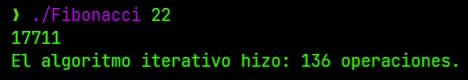
\includegraphics[width=10cm,height=5cm]{Fib_It_run.jpg}
        \end{picture}
    \end{figure}
    \vspace{-0.7cm}
    \begin{center}
        Figura 1. Ejecución de FibonacciIterativo
    \end{center}
    \medskip
\newpage
A continuación haremos su análisis a $priori$:
\begin{figure}[h]
    \vspace{3cm} \hspace{-2cm} \setlength{\unitlength}{1mm}
        \begin{picture}(15,25)(-35,0)
            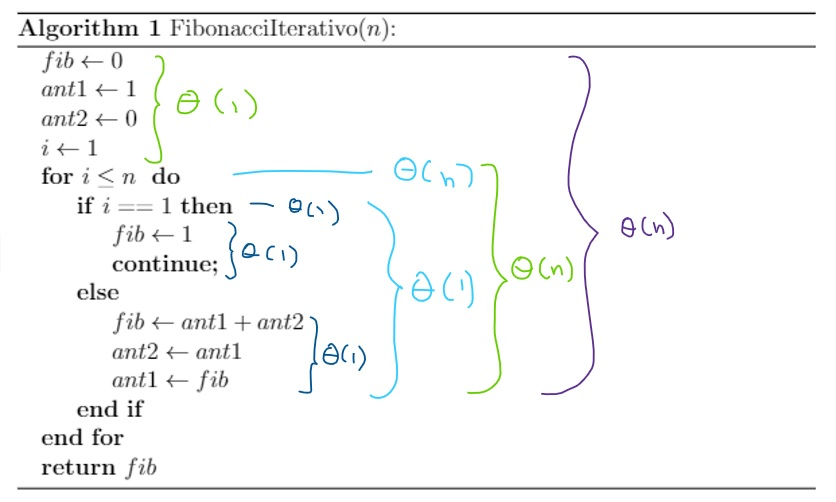
\includegraphics[width=10cm,height=5cm]{Fib_It_priori.jpg}
        \end{picture}
    \end{figure}
    \vspace{-0.7cm}
    \begin{center}
        Figura 2. Análisis a $priori$ de FibonacciIterativo
    \end{center}
    \medskip
De aquí podemos ver que FibonacciIterativo $\in O(n)$.
\newline
\\ A manera de comprobación checaremos su análisis a $posteriori$:
\begin{table}[htbp]
    \begin{center}
        \begin{tabular}{|c|c|}
            \hline
            \textbf{n} & \textbf{\# operaciones} \\
            \hline \hline
            0 &	6 \\ \hline
            1 & 10 \\ \hline
            2 &	16 \\ \hline
            3 &	22 \\ \hline
            4 &	28 \\ \hline
            5 &	34 \\ \hline
            6 & 40 \\ \hline
            7 & 46 \\ \hline
            8 & 52 \\ \hline
            9 & 58 \\ \hline
            10 & 64 \\ \hline
        \end{tabular}
        \caption{Mediciones para FibonacciIterativo}
        \label{tabla:analisis1}
    \end{center}
\end{table}
\\Graficando estos valores tenemos lo siguiente:
\newpage
\begin{figure}[h]
    \vspace{3cm} \hspace{-2cm} \setlength{\unitlength}{1mm}
        \begin{picture}(15,25)(-35,0)
            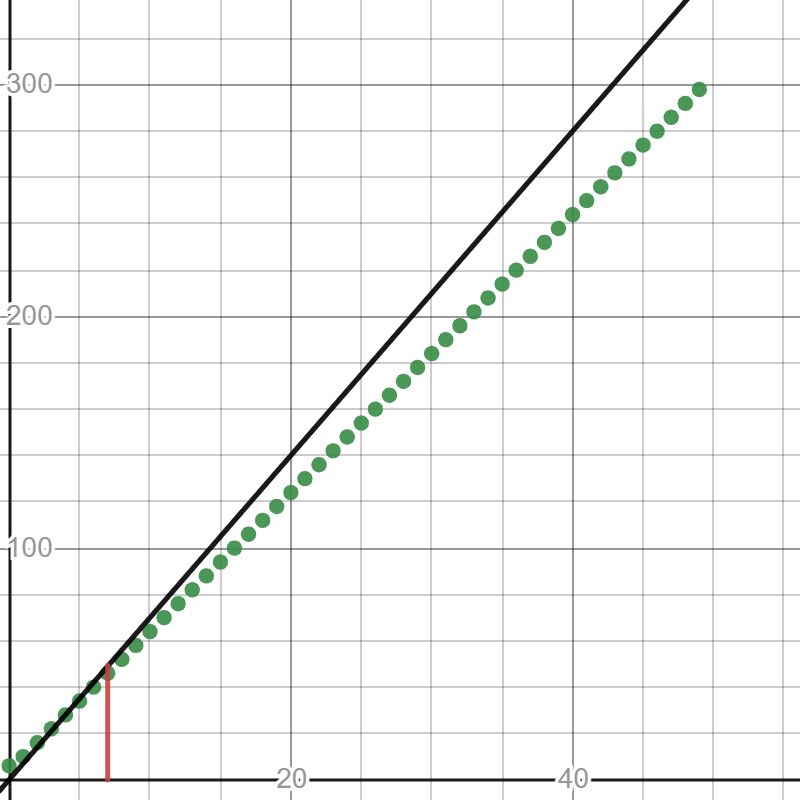
\includegraphics[width=10cm,height=5cm]{It_Fib_post.png}
        \end{picture}
    \end{figure}
    \vspace{-1cm}
    \begin{center}
        Figura 3. Gr\'afica de la funci\'on $f(n) = 7n$
    \end{center}
    \medskip
    Podemos observar que algunos puntos están por encima, otros pasan por la recta, y finalmente otros están por debajo. De la definición de $O$:
    \\ Necesitamos encontrar un $c_1g(n) \geq 7n$  $\forall n \geq n_1$, de ah\'i que:
    \\ $7n \le 8n $ $\forall n \geq 7$, entonces $c_1 = 8$, $g(n)=n$, y $n_1=7$ $\therefore$ $f(n)=7n \in O(n)$.
    \\ Así comprobamos que el análisis a $priori$ y el a $posteriori$ coinciden. Así que podemos confirmar que FibonacciIterativo $\in O(n)$.
\newline
\\Ahora veamos este algoritmo en ejecución para su caso recursivo:
\begin{figure}[h]
    \vspace{3cm} \hspace{-2cm} \setlength{\unitlength}{1mm}
        \begin{picture}(15,25)(-35,0)
            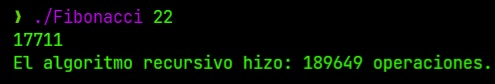
\includegraphics[width=10cm,height=5cm]{Fib_Rec_run.jpg}
        \end{picture}
    \end{figure}
    \vspace{-0.9cm}
    \begin{center}
        Figura 4. Ejecución de FibonacciRecursivo
    \end{center}
    \medskip
Ahora veremos el análisis a $posteriori$ de FibonacciRecursivo
\begin{table}[htbp]
    \begin{center}
        \begin{tabular}{|c|c|}
            \hline
            \textbf{n} & \textbf{\# operaciones} \\
            \hline \hline
            0 &	2 \\ \hline
            1 & 3 \\ \hline
            2 &	11 \\ \hline
            3 &	20 \\ \hline
            4 &	37 \\ \hline
            5 &	63 \\ \hline
            6 & 106 \\ \hline
            7 & 175 \\ \hline
            8 & 287 \\ \hline
            9 & 468 \\ \hline
            10 & 761 \\ \hline
        \end{tabular}
        \caption{Mediciones para FibonacciRecursivo}
        \label{tabla:analisis2}
    \end{center}
\end{table}
\newpage
Graficando estos valores tenemos la siguiente gráfica:
\begin{figure}[h]
    \vspace{3cm} \hspace{-2cm} \setlength{\unitlength}{1mm}
        \begin{picture}(15,25)(-35,0)
            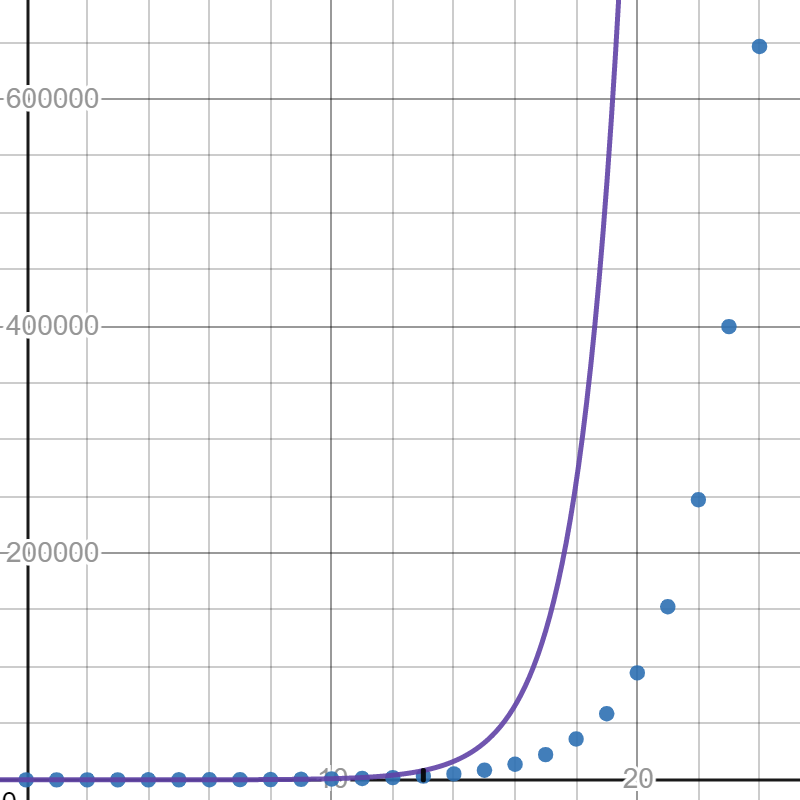
\includegraphics[width=10cm,height=5cm]{Rec-Fib-post.png}
        \end{picture}
    \end{figure}
    \vspace{-1cm}
    \begin{center}
        Figura 5. Gr\'afica de la funci\'on $f(n) = 2^n$
    \end{center}
    \medskip
    Podemos observar que algunos de estos puntos pasan por la función, y los demás están por debajo. De la definición de $O$:
    \\ Necesitamos encontrar un $c_1g(n) \geq 2^n$  $\forall n \geq n_1$, de ah\'i que:
    \\ $2^n \le 2^{n+1} $ $\forall n \geq 13$, entonces $c_1 = 2$, $g(n)=2^n$, y $n_1=13$ $\therefore$ $f(n)=2^n \in O(2^n)$.
\\Ahora si comparamos FibonacciIterativo v.s. FibonacciRecursivo, podemos ver que la diferencia es mucha, puesto que la versión iterativa, tiene una $T(n)$ polinomial, sin embargo la versión recursiva no. Podemos concluir que Fibonacci corresponde a un problema de la clase $P$, puesto que existe una solución que lo resuleva en tiempo polinomial.
\newpage
Ahora vamos a ver nuestro segundo problema, es decir, el de los n-primeros números perfectos.
Ya que lo separamos en 2 casos, vamos a ver primero Perfecto, así que a continuación se muestra en ejecución este algoritmo:
\begin{figure}[h]
    \vspace{3cm} \hspace{-2cm} \setlength{\unitlength}{1mm}
        \begin{picture}(15,25)(-35,0)
            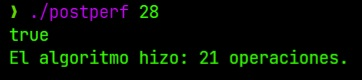
\includegraphics[width=10cm,height=5cm]{Perf_run.jpg}
        \end{picture}
    \end{figure}
    \vspace{-0.9cm}
    \begin{center}
        Figura 6. Ejecución de Perfecto
    \end{center}
    \medskip
En seguida se muestra el análisis a $priori$ de Perfecto
\begin{figure}[h]
    \vspace{3cm} \hspace{-2cm} \setlength{\unitlength}{1mm}
        \begin{picture}(15,25)(-35,0)
            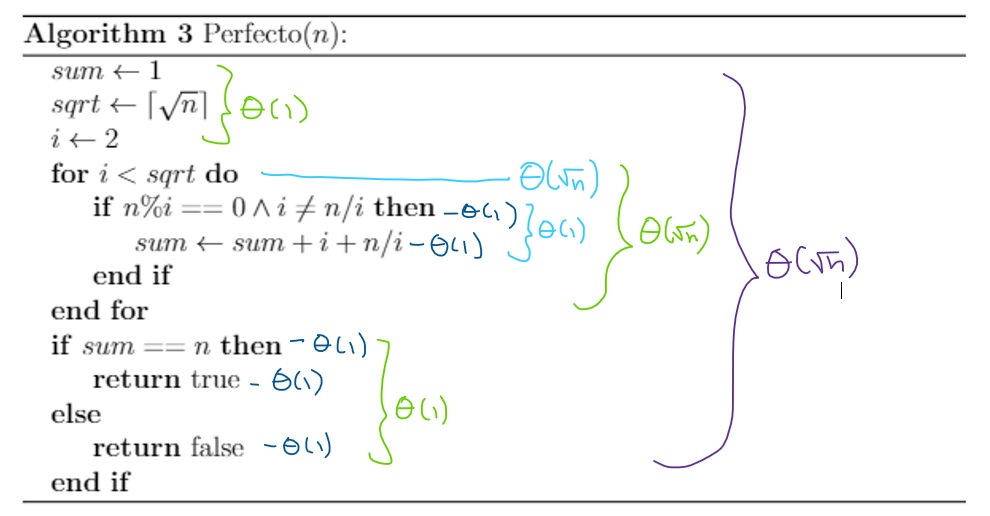
\includegraphics[width=10cm,height=5cm]{Perf_priori.jpg}
        \end{picture}
    \end{figure}
    \vspace{-0.9cm}
    \begin{center}
        Figura 7. Análisis a $priori$ de Perfecto
    \end{center}
    \medskip
La línea del for es $O(\sqrt{n})$ porque requerimos que $i$ sea mayor o igual a $\sqrt{n}+1$, por ende se ejecuta $O(\sqrt{n})$. Finalmente podemos decir que Perfecto $\in O(\sqrt{n})$.
\newpage
Posteriormente veremos el análisis a $posteriori$ de Perfecto
\begin{table}[htbp]
    \begin{center}
        \begin{tabular}{|c|c|}
            \hline
            \textbf{n} & \textbf{\# operaciones} \\
            \hline \hline
            0 &	5 \\ \hline
            1 & 5 \\ \hline
            2 &	5 \\ \hline
            3 &	5 \\ \hline
            4 &	5 \\ \hline
            5 &	8 \\ \hline
            6 & 10 \\ \hline
            7 & 8 \\ \hline
            8 & 10 \\ \hline
            9 & 8 \\ \hline
            10 & 13 \\ \hline
            20 & 18 \\ \hline
            30 & 23 \\ \hline
            40 & 26 \\ \hline
            50 & 32 \\ \hline
        \end{tabular}
        \caption{Mediciones para Perfecto}
        \label{tabla:analisis3}
    \end{center}
\end{table}
\\Graficando estos valores tenemos la siguiente gráfica:
\begin{figure}[h]
    \vspace{3cm} \hspace{-2cm} \setlength{\unitlength}{1mm}
        \begin{picture}(15,25)(-35,0)
            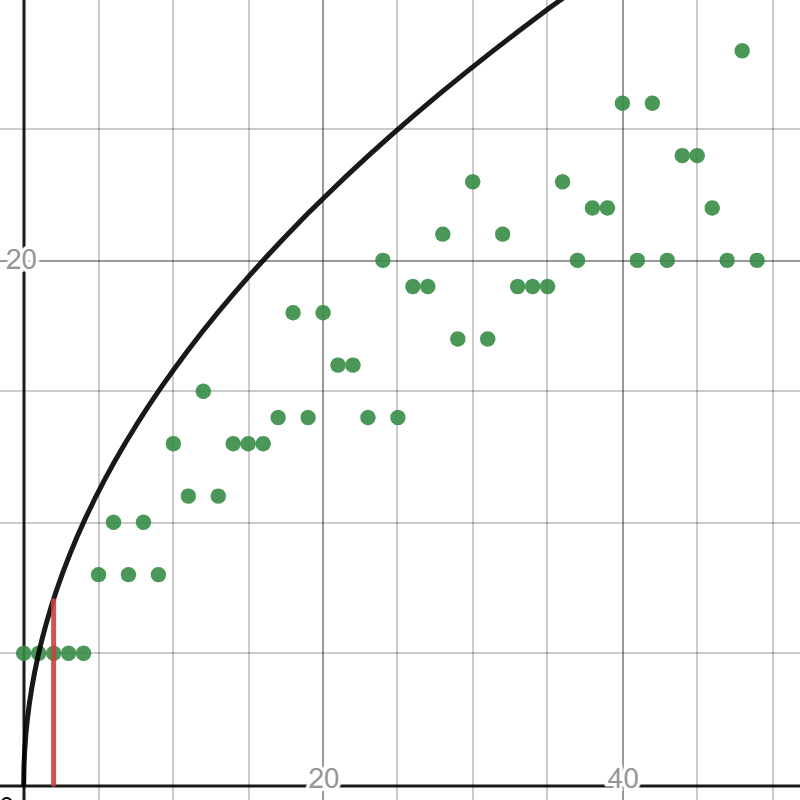
\includegraphics[width=10cm,height=5cm]{Perf_post.png}
        \end{picture}
    \end{figure}
    \vspace{-1cm}
    \begin{center}
        Figura 8. Gr\'afica de la funci\'on $5\sqrt{n}$
    \end{center}
    \medskip
    Podemos observar que algunos de estos puntos pasan por la función, y los demás están por debajo. De la definición de $O$:
    \\ Necesitamos encontrar un $c_1g(n) \geq 5\sqrt{n}$  $\forall n \geq n_1$, de ah\'i que:
    \\ $5\sqrt{n} \le 6\sqrt{n} $ $\forall n \geq 2$, entonces $c_1 = 5$, $g(n)=\sqrt{n}$, y $n_1=2$ $\therefore$ $f(n)=5\sqrt{n}\in O(\sqrt{n})$. Por lo tanto podemos decir que Perfecto $\in O(\sqrt{n})$.
\newpage
Con esto podemos ahora sí ejecutar nuestro algoritmo completo para encontrar los n-números perfectos. Así se ve ejecutandose:
\begin{figure}[h]
    \vspace{3cm} \hspace{-2cm} \setlength{\unitlength}{1mm}
        \begin{picture}(15,25)(-35,0)
            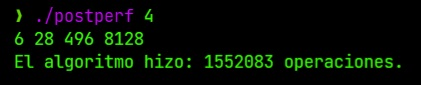
\includegraphics[width=10cm,height=5cm]{NPerf_run.jpg}
        \end{picture}
    \end{figure}
    \vspace{-0.9cm}
    \begin{center}
        Figura 9. Ejecución de MostrarPerfectos
    \end{center}
    \medskip
Finalmente vamos a checar el análisis a $posteriori$ de MostrarPerfectos
Ya que nuestra computadora solo fue capaz de mostrar los primeros 5 números perfectos, se adjuntan dichas mediciones.
\begin{table}[htbp]
    \begin{center}
        \begin{tabular}{|c|c|}
            \hline
            \textbf{n} & \textbf{\# operaciones} \\
            \hline \hline
            1 &	20 \\ \hline
            2 & 407 \\ \hline
            3 &	25956 \\ \hline
            4 &	1552083 \\ \hline
            5 &	389301767021 \\ \hline
        \end{tabular}
        \caption{Mediciones para MostrarPerfectos}
        \label{tabla:analisis4}
    \end{center}
\end{table}
\newpage
Graficando estos valores tenemos la siguiente gráfica:
\begin{figure}[h]
    \vspace{3cm} \hspace{-2cm} \setlength{\unitlength}{1mm}
        \begin{picture}(15,25)(-35,0)
            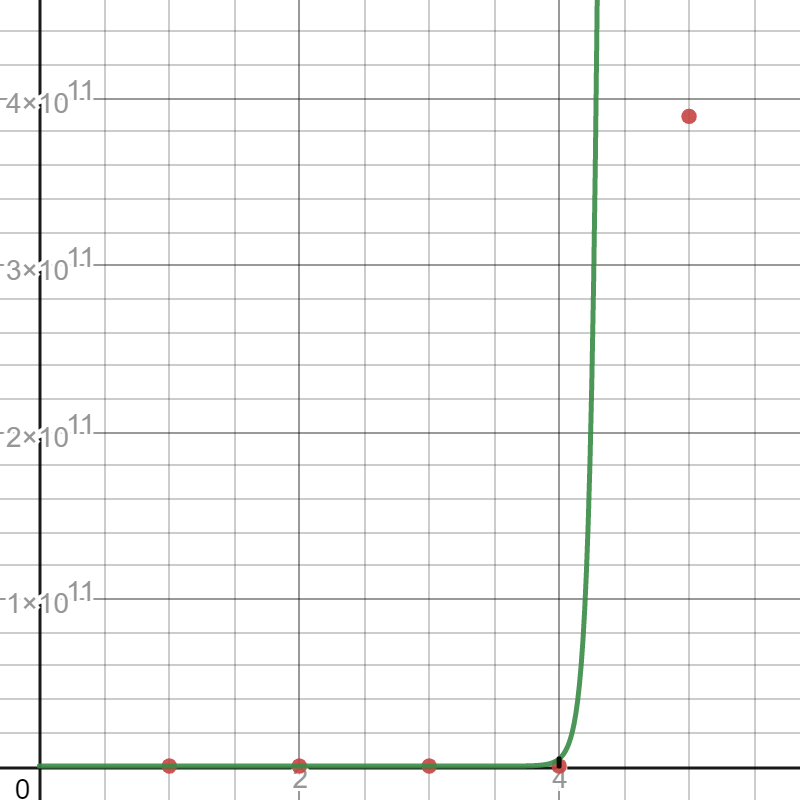
\includegraphics[width=10cm,height=5cm]{NPerf_post.png}
        \end{picture}
    \end{figure}
    \vspace{-0.8cm}
    \begin{center}
        Figura 10. Gr\'afica de la funci\'on $n^{n^2}$
    \end{center}
    \medskip
    Podemos observar que algunos de estos puntos pasan por la función, y los demás están por debajo. De la definición de $O$:
    \\ Necesitamos encontrar un $c_1g(n) \geq n^{n^2}$  $\forall n \geq n_1$, de ah\'i que:
    \\ $n^{n^2} \le 2n^{n^2} $ $\forall n \geq 4$, entonces $c_1 = 2$, $g(n)=n^{n^2}$, y $n_1=4$ $\therefore$ $f(n)=n^{n^2} \in O(n^{n^2})$. Por lo tanto podemos decir que MostrarPerfectos $\in O(n^{n^2})$.
\\ Por lo que podemos observar que aunque nuestra función Perfecto $\in O(\sqrt{n})$, nuestra computadora no fue capaz de encontrar más de 5 números perfectos, a pesar de que estuvo 10 horas tratando de encontrarlo, puesto que no está acotada por un polinimio, y si no existiera una función de MostrarPerfectos que lo hiciera en tiempo polinomial, podríamos concluir que es un problema que pertenece a la clase $NP$, pero como no sabemos entonces lo dejaremos en la clase $NPC$. 
\newpage
\section{Conclusiones}
\textbf{Conclusi\'on General}
\\Fue complicado escribir la versión iterativa de Fibonacci, puesto que no se lograba apreciar que debía actualizarse inmediatamente el anterior1 con el Fibonacci actual, luego un error que se presentó fue que al hacer el análisis a posteriori de la versión recursiva de Fibonacci, me di cuenta que estaba regresando la versión iterativa en vez de la recursiva. Quizás para mejorar se pudieran checar mejor las condiciones de la versión iterativa, o incluso ocupar alguna fórmula matemática. Se obtuvieron los resultados esperados, aunque se esperaba que la computadora donde se probaron los algoritmos fuera capaz de obtener al menos 6 números perfectos.
\newline
\newline
\textbf{Conclusi\'on de Anthony}

\begin{wrapfigure}{r}{5.5cm}
    
\includegraphics[width=5.5cm]{me.jpg}
\end{wrapfigure} 
En lo particular me agrada que los problemas que se estén resolviendo tengan que ver con matemáticas, puesto que en lo personal me parece interesante, además es curioso, el cómo uno espera cierto comportamiento del código que se está escribiendo. Además, ahora con el uso de programas auxiliares, para generar archivos que nos permitan obtener más fáciles los datos para el análisis a $posteriori$ resultó bastante atractivo, y mucho más eficiente. Finalmente, resulta imperativo recalcar que es mucho más fácil calcular la complejidad de un algoritmo mediante el análisis a $priori$, bueno cuando se pueden ocupar los teoremas y las reglas expuestas en este trabajo, porque a línea por línea, resulta bastante tardado, y a veces hasta complicado.
\newpage
\section{Anexo}
Para este caso no se realizaron problemas de tarea para anexar.

\section{Bibliograf\'ia}

Cormen, T. H., \& Cormen, T. H. (2001). Introduction to algorithms. Cambridge, Mass: MIT Press.
\newline
Karumanchi, N, (2017). Data Structures and Algorithms Made Easy - Data Structures and Algorithmic Puzzles. Career Monk.
\newline
Rubio-Sanchez, M, (2018). Introduction to Recursive Programming. CRC Press.

\medskip

\end{document}